% Chapter Template

\chapter{Introduction} % Main chapter title

\label{ch:Introduction} % Change X to a consecutive number; for referencing this chapter elsewhere, use \ref{ChapterX}

\lhead{\emph{Introduction}} % Change X to a consecutive number; this is for the header on each page - perhaps a shortened title

%----------------------------------------------------------------------------------------
%	INTRO TEXT
%----------------------------------------------------------------------------------------


The \textbf{user interface}, or human-computer interface, is the component of a computer system that provides a space of interaction between the human user and the resources offered by the machine; such a space defines a bridge language which human intentions can be translated into, to be converted into computational procedures for the machine; vice versa, the result of the computation is then presented to the user in the same language, which he or she is assumed to understand.

% cite Tanenbaum
In the early days of computing, the so-called \textbf{batch interfaces} were non-interactive: the user/programmer was supposed to feed the machine with a software, punched on cards using the \textit{machine's assembly language} directly, and retrieve the result of the computation printed on paper. The third and fourth generations of computing brought \textbf{text-based} interfaces for operating systems (UNIX, DOS, CP/M), that were later taken over by \textbf{Graphical User Interfaces} (GUI), moving the human-machine interaction on a new, visual language made of windows, icons and buttons. Recently, touch screen and camera devices allowed for the implementation of even more natural means of interaction based on visual and \textbf{haptic} technologies.

From this brief spot on computing history, and in a way from common sense, we can draw the rather trivial, yet crucial, conclusion that the trend in user interfaces development is to \textbf{close the gap} between humans and machines by moving the needle of the interface languages from a machine-centered space towards the human language itself. Due to this, the studies on Natural Language Processing (NLP) assume a dramatically central role, as dramatically central is natural language in the interaction of humans with each other.

For this reason, the focus of this thesis work concerns the area of \textbf{dialogue systems}.

%----------------------------------------------------------------------------------------
%	DIALOGUE SYSTEMS
%----------------------------------------------------------------------------------------
\section{Dialogue Systems}\label{ch:introduction:ds}
Research on dialogue systems has been carried on since the \textbf{early days} of Artificial Intelligence. A milestone in the early work on this field is ELIZA \citep{Weizenbaum:1966:ECP:365153.365168}, which provides the user with a basic human-like interaction based on pattern matching; Figure \ref{ch:rw:ds:ELIZA} shows an instance of these patterns.

Another example is the SHRDLU system \citep{winograd1971procedure}, which interfaces the user with a simple spatial domain by listening to the user's utterances (e.g.\ ``Would you please put the green pyramid in the box?"), and performing actions accordingly in the domain, resolving, if necessary, ambiguous or implicit references to the entities in it.

\begin{figure}
\begin{Verbatim}[frame=single]
["dream", 3, [
 ["*", [
     "What does that dream suggest to you ?",
     "Do you dream often ?",
     "What persons appear in your dreams ?",
     "Do you believe that dreams have something to do
      with your problem ?"
  ]]
]]
\end{Verbatim}
\caption{One of the patterns included in ELIZA's DOCTOR script. It simply tells the system that the user input can be answered with any of the given sentences, whenever it contains the word ``dream".}
\label{ch:rw:ds:ELIZA}
\end{figure}

According to \cite{Jokinen2009}, modern dialogue systems can be divided in \textbf{two main types}: task-oriented and nontask-oriented. Intuitively, systems in the first category are meant to deal with a specific task such as making a hotel booking, or booking a plane ticket; an example in this category is the MIT Mercury system, a vocal interface to a flight database \citep{Seneff:2000:DMM:1605285.1605288}. On the other hand, nontask-oriented systems are meant to engage in conversations without a specific purpose to fulfill, but the one of delivering a realistic simulation; ELIZA itself is an example of nontask-oriented dialogue system.

Task-oriented systems can be very simple, as simple and well-formalized the task is;  many applications, such as travel service or call routing, can be successfully solved by \textbf{slot-based} systems: each step of the conversation requires some pieces of information, modeled as slots, to be filled in by the user (departure city, arrival city, date, and so on); given the slots to be filled, the dialogue task can be solved with a formal grammar of interaction. As the complexity increases, more phenomena of human interaction have to be modeled, such as turn-taking, multimodality or grounding
%\ignore{CITE RAQUEL'S CHAPTER}
, as well as semantic structures such as quantification and negation; slot-based systems are not sufficient to model these scenarios \citep{Gabsdil03clarificationin}, that require more advanced frameworks such a the Information State Update (ISU) one, which will be tackled in \ref{ch:rw:ds:isu}.


%----------------------------------------------------------------------------------------
%	DIALOGUE SYSTEMS
%----------------------------------------------------------------------------------------

\section{General Architecture of a Dialogue System} \label{ch:introduction:arch}
A dialogue system, or conversational agent (CA), is a computer software that allows humans and machines to interact through an intermediate language which is as close as possible to the \textbf{human language}, and through conversational episodes that implement as close as possible the human dialogue modalities.

The \textbf{basic architecture} of a dialogue system is shown in Figure \ref{ds_arch}. The figure represents the flow of information during the interaction between the system and a human user.

\begin{figure}
	\centering
	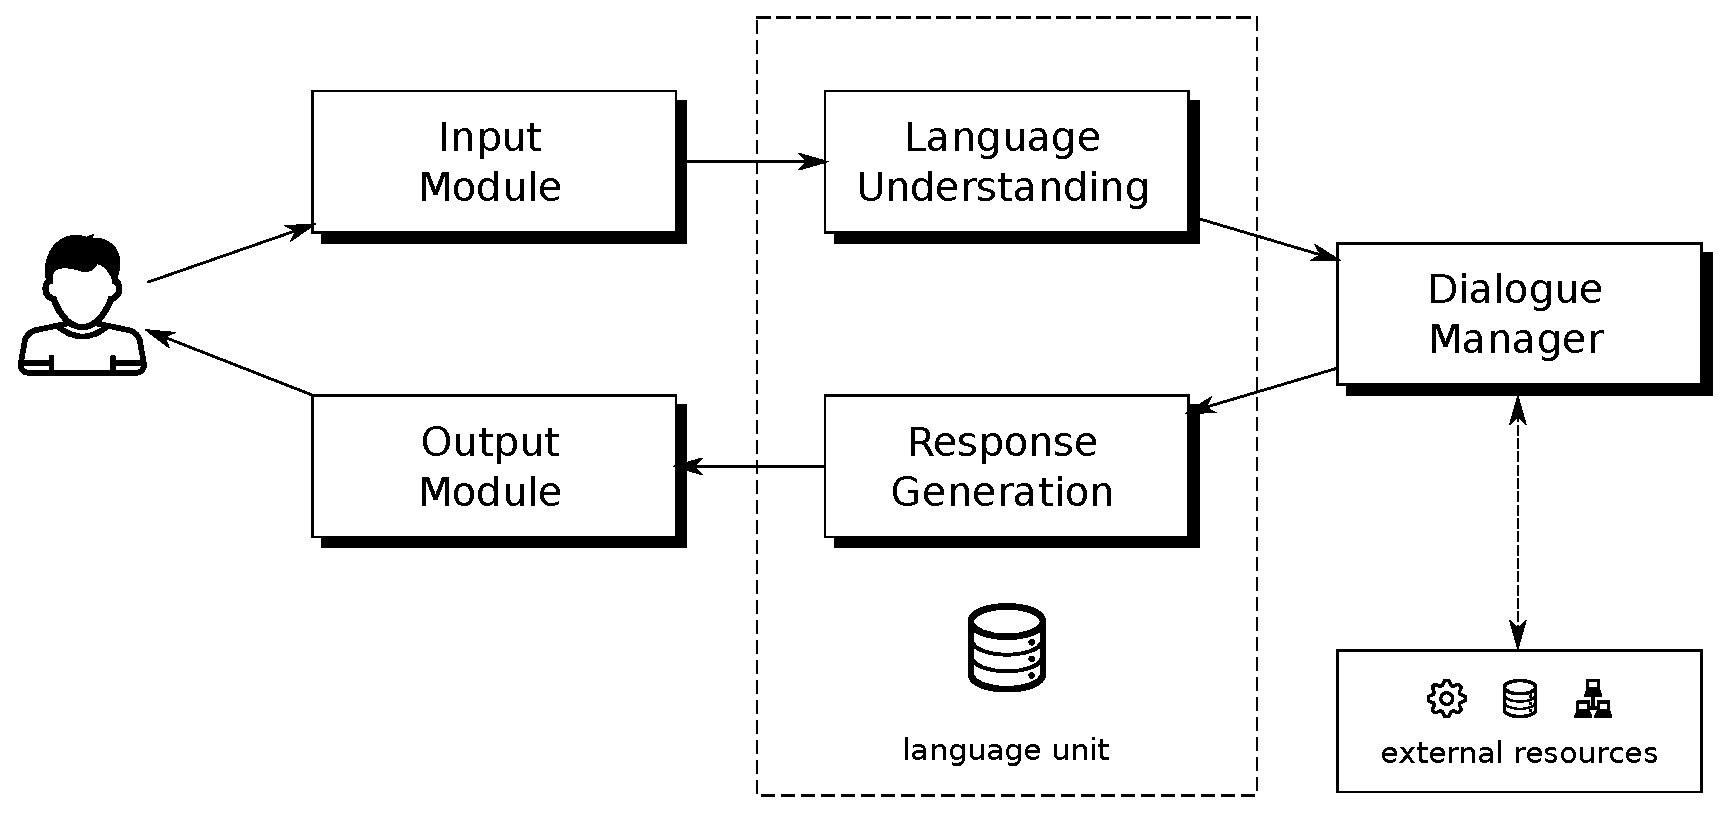
\includegraphics[width=15cm]{Pictures/ds_arch.pdf}
	\caption{The basic architecture of a dialogue system}
	\label{ds_arch}
\end{figure}
 
 \begin{enumerate}
	\item The user produces an utterance to be entered in the system, that receives it through its \textbf{input module}. As an example, the user may start a conversation by asking \textit{``What's your name?"}. Note that, although we will only address text-based interaction, spoken dialogue systems exist, where the input module is an Automatic Speech Recognition software.
	\item The \textbf{language understanding} module receives the user utterance, and interprets it into a logical form that the system can work with. In the previous example, the language understanding module would receive the string \texttt{"What's your name"} as input, and will output a formal representation of the dialogue act performed by the utterance, for instance something like \texttt{"ask(?X.my\_name(X))"}.
	\item The result of the interpretation is given to the \textbf{dialogue manager} (DM). This component is the core of the system, as it has to model and keep track of the dialogue context and, within this context, integrate the user moves and plan the system responses. The dialogue manager can also access external resources in order to satisfy the user requests. In the example, the DM receives the interpreted user move \texttt{"ask(?X.my\_name(X))"}; its will then process this information, which broadly means:
	\begin{enumerate}
		\item Update the context, to include the pending user request.
		\item Find an answer for the user request
		\item Output the answer in the form of a system move (in the example, \\ \texttt{"answer(my\_name(`HAL9000'))"})
	\end{enumerate}
	\item The system move is received by the \textbf{response generation} module, whose purpose is to express that move with a natural language sentence, In the example, a proper output would be the string \texttt{"My name is HAL9000"}.
	\item Finally, the response string is received by the \textbf{output module}, which presents it to the user. This module can simply print the sentence on the screen, but it can also implement Text-To-Speech technology to allow spoken interaction with the user.
\end{enumerate}

As we will see in the next chapters, our work will be focused on the language understanding and response generation modules, that together form what we call the \textbf{Language Unit}. Our goal is to implement advanced language understanding and learning capabilities for this part of the system. As a part of the learning capabilities of the system involves interaction with the user (see Section \ref{ch:rw:ds:grounding}), the dialogue manager was also extended to support such interaction (see Chapter \ref{ch:interaction}).


%----------------------------------------------------------------------------------------
%	LEARNING TO TALK
%----------------------------------------------------------------------------------------

\section{Learning to talk}

One of the constituent features of humans' ability to speak is that such an ability doesn't come fully developed in children, but rather \textbf{grows} with time, influenced by the interaction of the subject with the outer world.
%~ One of the constituent features of humans' ability to speak is that such an ability is \textbf{not innate}, but is rather learned through interactions.

Ever since the power of computers grew enough to allow for intensive statistical analysis of significant amounts of data, \textbf{Machine Learning} approaches to Artificial Intelligence tasks got more and more prominent in the scene, often outperforming static methods (i.e. where the solution procedure for a task is explicitly coded by the programmer).
% Citation needed...
One of the clearest examples is the field of NLP itself, where the most important tasks, like parsing or machine translation, are dominated by Machine Learning methods based on corpora,
% Citation needed
meaning that, for instance, a Machine Translation system will first be trained on a corpus of aligned sentences. Statistical structures will be extracted from this corpus, like the most likely word-by-word alignment, and later be used to process new examples.

However, the task of learning through dialogue interactions comes with some \textbf{peculiar} challenges. First of all, humans learning to talk do not go through two separate phases of learning and processing, but rather improve their abilities episode by episode; as \cite{2095408} point out, this \textbf{incremental learning} structure is nowadays not implemented in state-of-the-art systems. Also, the nature of this incrementing learning is \textbf{not linear}, as the new information was stacked little by little on the existing one: new words and phrases can be described with concepts and linguistic structures that are already present in the learner's mind. Lastly, if we keep considering the way humans learn to talk, we realize that, as from a certain point, the language ceases to be a mere subject of learning, and \textbf{becomes the means} by which it is itself learned: the same linguistic structures that are used to express concepts and categories of the learner's experience, can also be used to describe themselves, as they become part of the same experience; we can observe a clear example of this process in any primary-school-level English class, where the teacher explains, by using English sentences, how English sentences are structured.

We can identify some \textbf{ideal features} we would like to have implemented into an automatic language learner:
\begin{itemize}
	\item Learning to produce or understand new surface forms, or \textbf{realizations}, for a given meaning -- eg. the sentence ``Bill eats an apple" for the action of Bill eating an apple.
	\item Learning to produce new \textbf{meanings} from the existing ones and their respective realizations -- eg. the concept of motor home, sharing the features of a house and a car.
	\item Learning a \textbf{``grammar" of conversation}, to place the correct utterance at each step of a conversational episode. -- eg. an appropriate answer to the utterance ``My name is Bill" can be ``Nice to meet you", whereas ``I like cookies" would not sound as much appropriate.
	%~ \item Learning to talk about its \textbf{meta} level, that is, the structures that control the production of utterances, like the syntax according to which new utterances are formed, or the ``grammar" of conversation of the previous point. 
\end{itemize}
Lastly, we can point out that when we talk of such things like \emph{realizations}, \emph{meanings} and \emph{episodes} we cannot provide exact, sharply bounded definitions, as it can be argued for \textbf{recursive and compositional} structures at any level of their interpretation. As an example, let's consider the sentence \enumsentence{I am pronouncing a sentence that contains two verbs and three nouns} The meaning of such a sentence describes structural elements of the sentence itself (which is the realization of the same meaning) and also the conversational episode that starts when the sentence is stated.

%----------------------------------------------------------------------------------------
%	THIS THESIS PROJECT
%----------------------------------------------------------------------------------------

\section{This thesis project} \label{ch:intro:project}

The aim of this thesis project is to design and implement language learning capabilities for an existing dialogue system, focusing on the \textbf{realization level}. That is, given a fixed list of meanings, the system should be able to classify every given sentence into its correct meaning. A client application has also been developed, that makes use of the dialogue system to solve a real user experience task.

Such an application is a voice-controlled music player, which has been named \textbf{\pname}. The task of such an application is to to get natural language input from the user and translate it into an appropriate corresponding behaviour. For example, when the input is ``Play Pictures at an exhibition", the system should start playing the famous suite by Modest Mussorgsky.

In this domain, each \textbf{meaning} corresponds to an action that the player can perform (e.g.\ play a song, jump to the next track, increase the volume, etc.), and is defined by a set of representative sentences, being its surface forms. For instance, the action of increasing the volume level can be defined by the following set of sentences:
\enumsentence{Increase the volume}
\vspace{-0.6cm}
\enumsentence{Increase the volume level}
\vspace{-0.6cm}
\enumsentence{Raise the volume}
\vspace{-0.6cm}
\enumsentence{Increase the volume please}

The \textbf{task} for the application is, given an arbitrary input sentence and a context (the point of the conversational episode being realized), to reply appropriately, and perform the correct action, that is, \textbf{associate} that sentence with its correct meaning. Furthermore, the system should be able to \textbf{learn} new realizations for each meaning, as unknown sentences are given in input and processed.

Note that such processing might be more or less \textbf{semantically intensive}. As an example, it can be argued that, given the above definition of the action to increase the volume, matching \textit{``Raise the volume please"} is an easier task than classifying \textit{``Turn up the volume"}. This is because the first sentence can be seen as a mere, string-wise, fusion of the two existing examples \textit{``Raise the volume"} and \textit{``Increase the volume please"}, whereas the second one requires a model of \textit{``Turn up"} being a string that carries the same meaning as other strings like \textit{``Increase"} or \textit{``Raise"}.

Also, an unknown input sentence should be given a \textbf{confidence score} for each candidate meaning it is associated to, in order for the system to model the uncertainty in the classification of unknown examples. This is important because, depending on the degree of confidence of an interpretation, the system may change its interaction plans (e.g.\ asking the user for clarification).

Finally, the system should be able to narrow possible needs for \textbf{clarification} down to single sentence components, eventually asking the user for disambiguation as specifically as possible. This is to enforce the learning of small components that may appear again in further unknown examples.

\subsection{Overview}

This work is structured as follows. Chapter \ref{ch:rw} reviews the \textbf{related work} that has been previously done; chapter \ref{ch:arch} describes the \textbf{architecture} of the solution that has been developed; chapter \ref{ch:M2} delves into the \textbf{M2 algorithm}, which is the core of the meaning matching feature of the application; chapter \ref{ch:interaction} describes how the system can learn though the \textbf{interaction} with the user; chapter \ref{ch:conclusions} draws the \textbf{conclusions} of the whole project and illustrates future work that could take steps from it.
